%!TEX root = ../plos_template.tex
\begin{figure}[!ht]
\centering
\noindent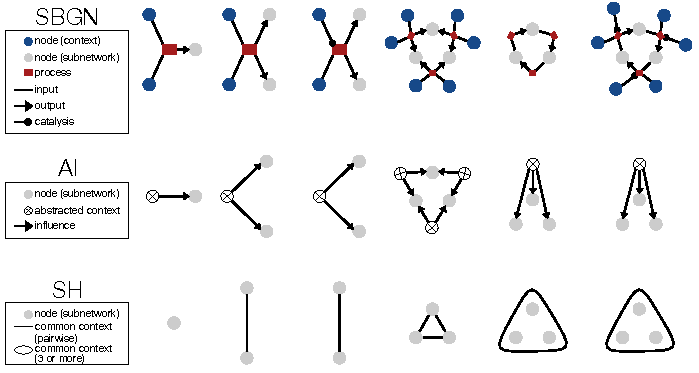
\includegraphics[width=0.9\columnwidth]{fig/netsubnetcontext.pdf}
\caption{{\bf Abstract influence representation of biological networks.} (row~1)~The systems biology graphical notation (SBGN) is capable of representing arbitrary biological networks including processes that involve metabolites, signaling molecules, genes, and enzymes \cite{LeNovere2009}. Only a fragment of the SBGN language, where all nodes have equivalent types, is indicated here. (row~2)~We abstract from the SBGN representation of a biological network to a graph representing the abstract influence (\AI{}) graph indicating coupling among a subset of the entities present in a biological network. (row~3)~For economy of representation we use a short hand (\SH{}) hypergraph to denote the \AI{} graph. The topology of the \AI{} and \SH{} graphs are equivalent and this is what we refer to as network architecture.}
\label{fig:netsubnetcontext}
\end{figure}

\begin{figure}[!ht]
\centering
\noindent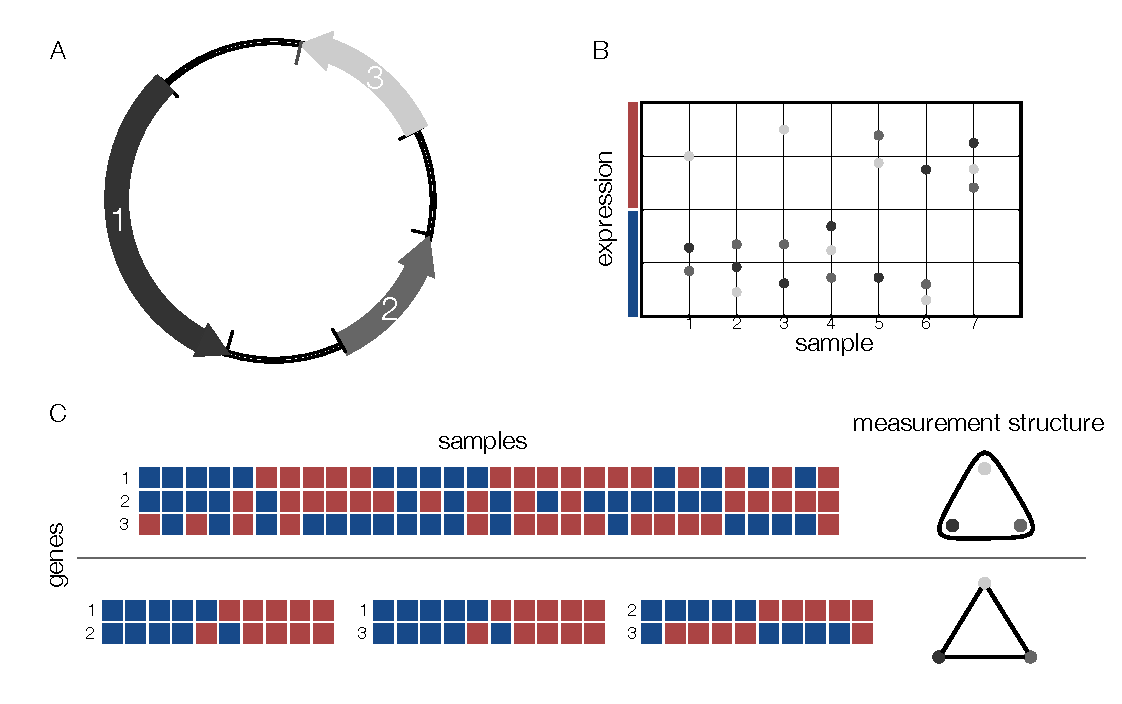
\includegraphics[width=0.9\columnwidth]{fig/figure_expression_concept.pdf}
\caption{{\bf Coarse-graining of biological network data.} (A) SBGN (top) and \SH{} (bottom) representation of two different biological networks. (B) Example binary coarse-graining of biological network data. For each sample a measurement is taken for all three variables in the focal subnetwork. The levels are binned into one of two classes represented by the red---- and blue bars representing relatively high and low levels respectively. (C) Heat map representation of coarse-grained data under the assumption of two different network architectures. The samples on top and the associated measurement structure correspond to the case where constraints are placed on all three variables by a single element of the network context (\autoref{fig:stochdynscheme} top row). The bottom represents the case where all three pairs are each independently constrained by elements of the network context (\autoref{fig:stochdynscheme} bottom row).}
\label{fig:expression_concept}
\end{figure}

\begin{figure}[!ht]
\centering
\noindent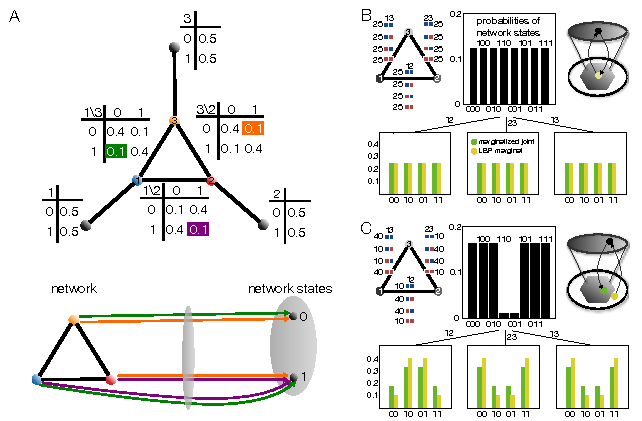
\includegraphics[width=0.9\columnwidth]{fig/inconsistentthreecycle.pdf}
\caption{{\bf Model of inconsistent network state data.} (A) An example structured according to the bottom row of \autoref{fig:expression_concept}C. The graph contains three nodes each representing one of the variables depicted in \autoref{fig:expression_concept}A. The dashed gray line coming from each variable points to the single variable marginal distribution depicted in the associated table. The pairwise edge marginal distributions are placed along the edges. The highlighted table entries (top) represent the constraint probabilities on the \gnpm{} represented by the equivalently colored arrows (bottom). The binary values representing variable states derive from the coarse-graining process over continuous network state data depicted in \autoref{fig:expression_concept}B. (B) (top-left) Representation of three hundred samples comprising a data set consistent with a uniform distribution over all \gnpm{} from the model in panel A. (top-middle) The joint probability distribution  given in the top-left panel. The green bars in the bottom three panels represent the marginalization of this joint distribution according to the structure of the graph. The yellow bars in the bottom three panels represent the ostensible marginal distributions determined via the sum-product algorithm (loopy belief propagation) \cite{Barber2012}. (top-right) A schematic where the top gray ellipse represents the space of joint probability distributions on three variables and the hexagon represents the pairwise marginals within their natural embedding space (see \autoref{fig:conediagram}).  For this data, maximum likelihood estimation (exact) and loopy belief propagation (approximate) yield equivalent points within the space of pairwise marginals. (C) Same as B, but with data consistent with \autoref{fig:expression_concept}C bottom, which in the limit of a large amount of data would converge to the ostensible node and edge marginal distributions in panel A. For the given data set, maximum likelihood estimation and loopy belief propagation yield different points within the natural embedding space of the pairwise marginals.}
\label{fig:inconsistentthreecycle}
\end{figure}


% determined via maximum-likelihood estimation with respect to the sufficient statistics (in this case, counts of pairwise observations of variables in states where blue corresponds to 0 and red corresponds to 1)

% The top-right panel is a schematic where the top gray ellipse represents the space of joint probability distributions on three variables each with two potential states (i.e. $\Delta_7$: the eight-dimensional probability simplex) and the bottom ellipse represents the union of three copies of the four-dimensional probability simplex (i.e. $\Delta_3^{\oplus 3}$)


\begin{figure}[!ht]
\centering
\noindent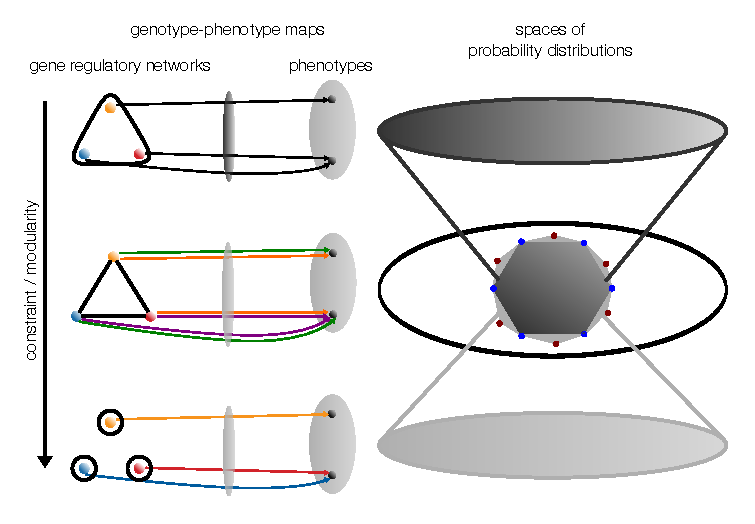
\includegraphics[width=0.9\columnwidth]{fig/conediagram.pdf}
\caption{{\bf Relationship between biological network models and spaces of probability distributions.} (A) The collection of all possible network architectures over three variables forms a lattice represented here by its Hasse diagram. An analogous lattice of network architectures exists for any number of variables. The Hasse diagram shows the manner in which network architectures are hierarchically related and are thus able to be embedded within one another. (B) Explicit examples of \gnpm{} over three network architectures from panel A highlighted in green are represented as arrows mapping the variables represented as nodes of the graph underlying the network architecture into the collection of network state values determined by the coarse-graining chosen in \autoref{fig:expression_concept}B. There is a different collection of possible \gnpm{} depending upon the structure of the network architecture. (C) Each collection of \gnpm{}, one representative for each network architecture depicted in panel B, is associated to a space of probability distributions defined over it. Moreover, the spaces of probability distributions associated to each graph are related via marginalization maps. The top level represents a joint probability distribution (i.e. $\Delta_7$: the eight-dimensional probability simplex) which can be marginalized to the middle space (i.e. $\Delta_3^{\oplus 3}$: the union of three copies of the four-dimensional probability simplex) which in turn can be marginalized to the bottom space (i.e. $\Delta_1^{\oplus 3}$: the union of three copies of the two-dimensional probability simplex). The light gray polytope in the middle, $\mathbb{L}(\mathcal{G})$, represents the space of distributions consistent with the marginalization map from the middle to the bottom. The dark gray polytope, $\mathbb{M}(\mathcal{G})$, represents the space of probability distributions consistent with marginalization from the top to the middle.}
\label{fig:conediagram}
\end{figure}

% \begin{figure}[!ht]
% \centering
% \noindent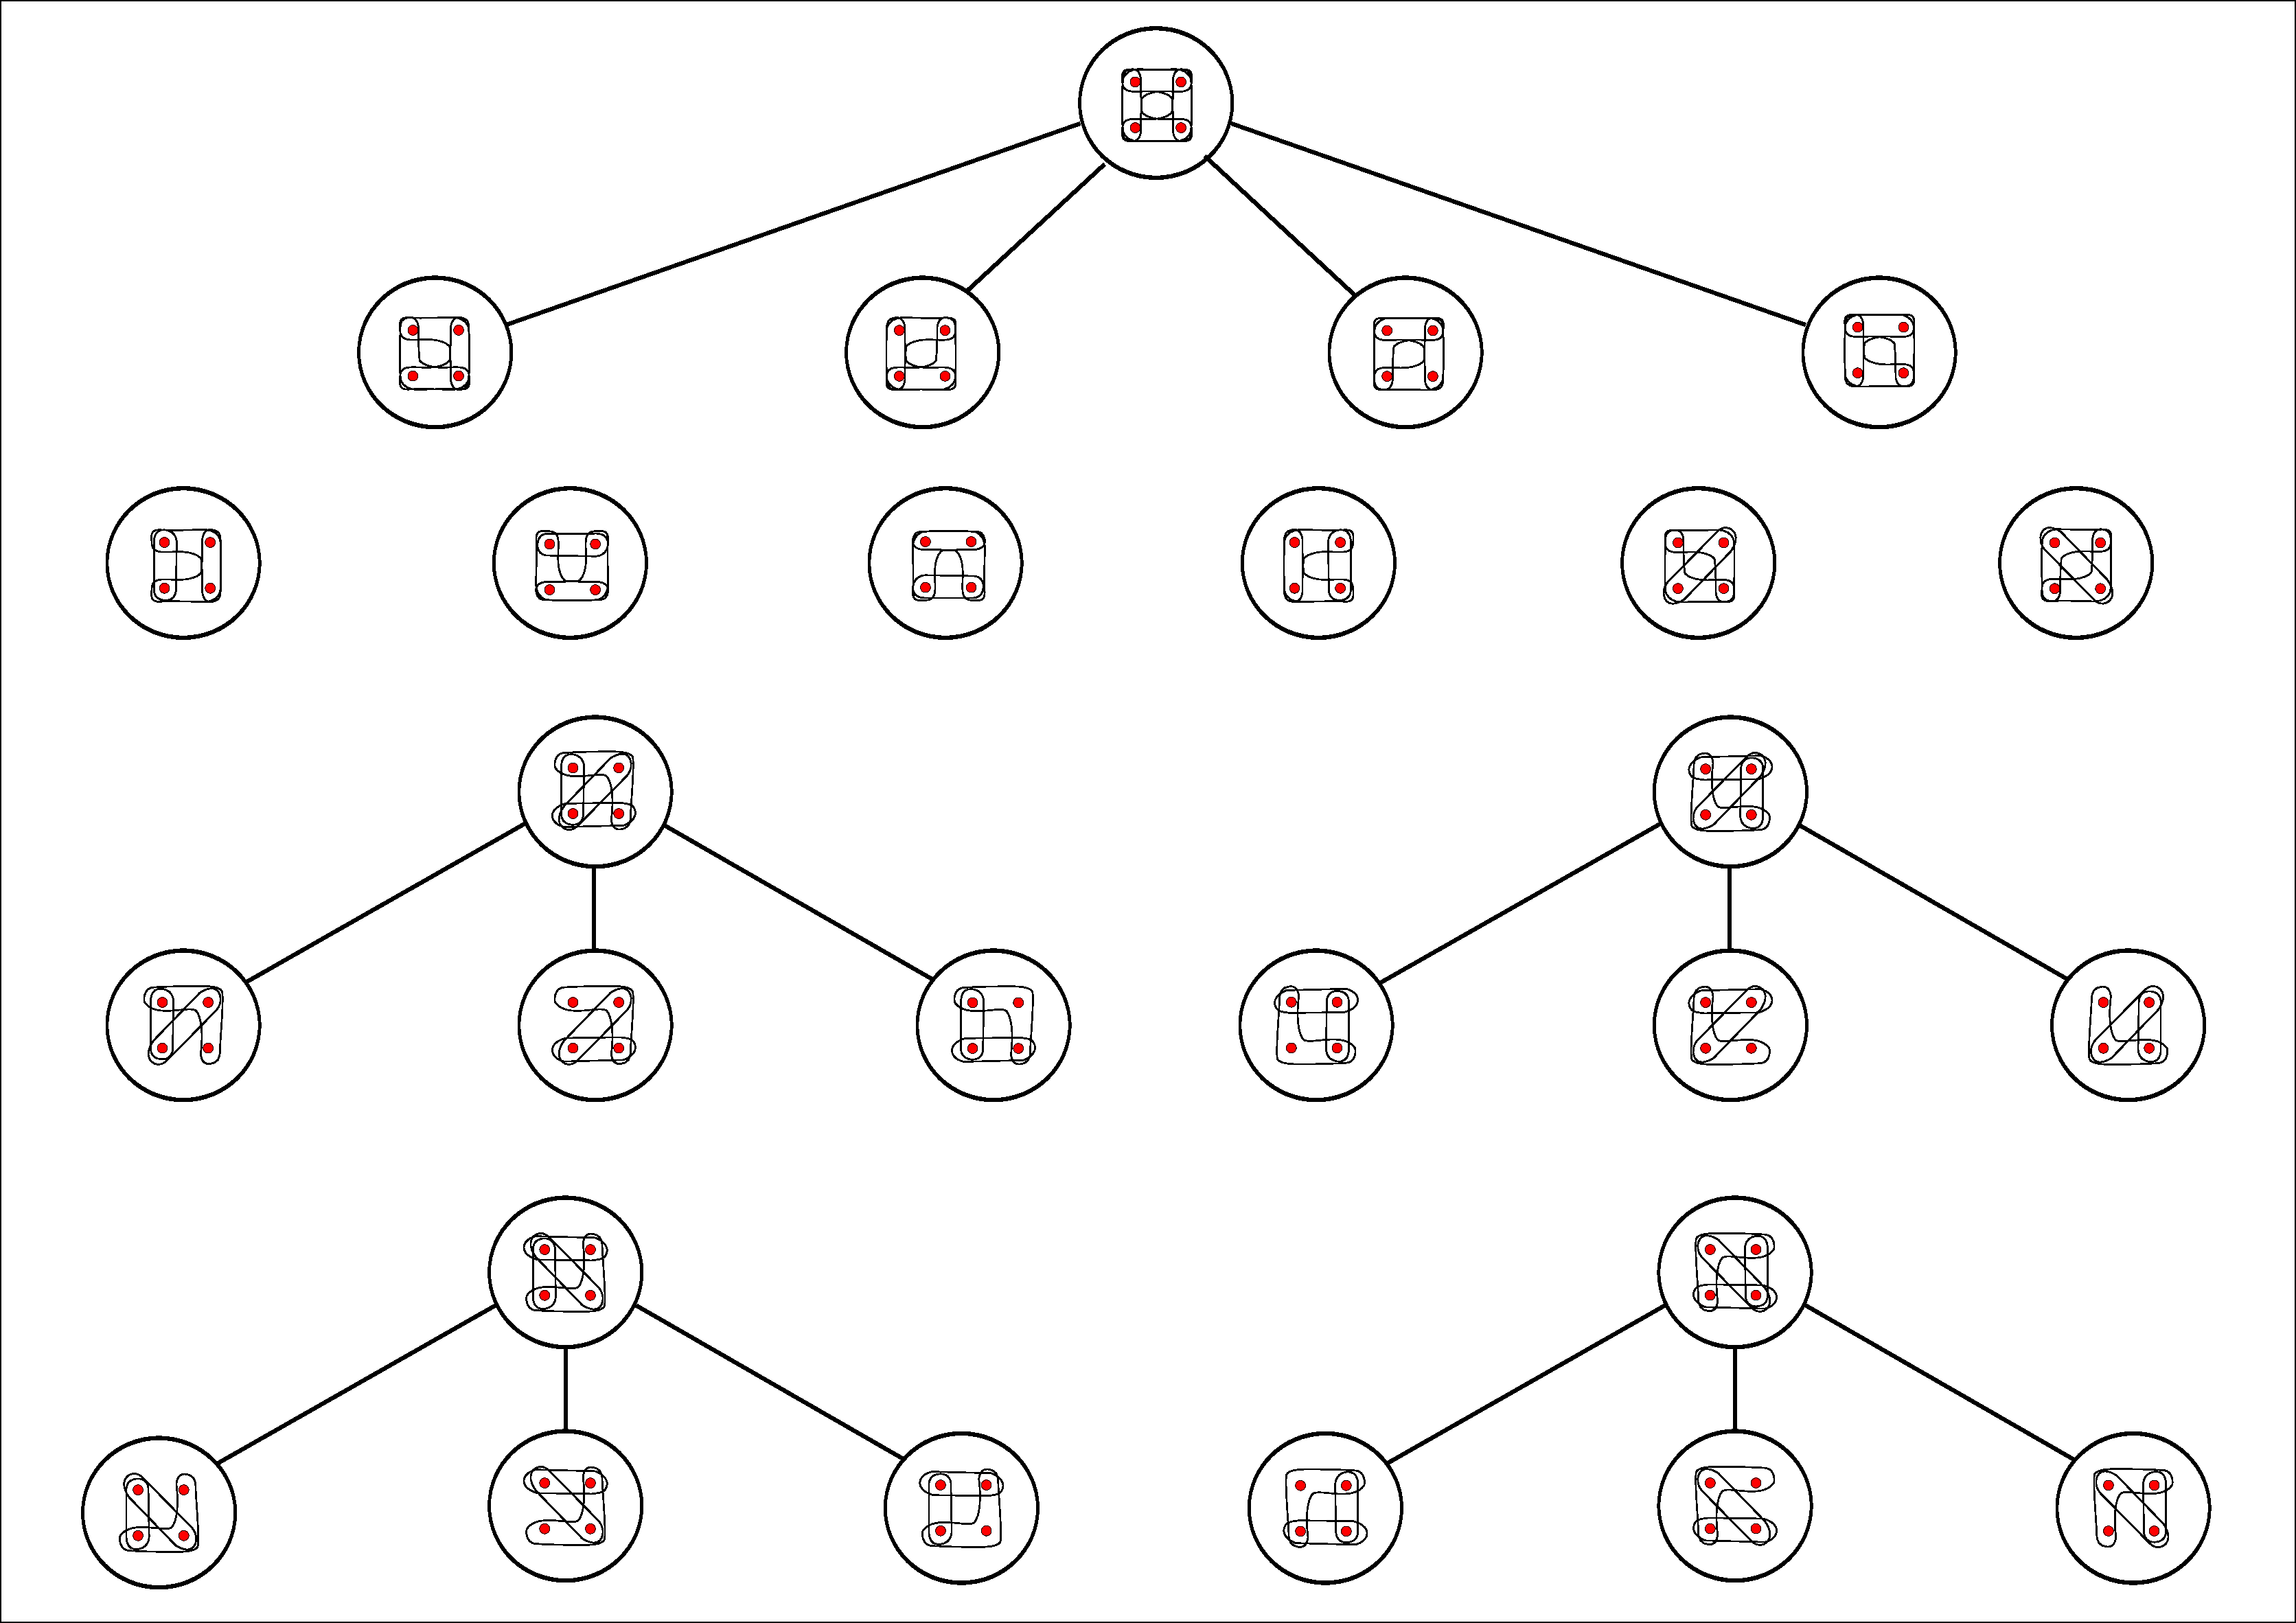
\includegraphics[width=1.0\columnwidth]{fig/non2uniformcyclichypergraphhasse.pdf}
% \caption{{\bf Hierarchical relationships among all possible classes of hypergraphs that are not graphs (i.e. not 2-uniform) but have cycles.} (A) There is a Hasse diagram for the lattice of GRNAs analogous to that of \autoref{fig:conediagram}A but defined on four rather than only three genes. Within this lattice some of the graphs have cycles and some do not. (B) The highest levels of the Hasse diagram associated to the lattice of GRNAs on four genes containing hypergraphs having cycles. (C) and (D) contain lower levels of GRNAs containing cycles. Each of the four panels in (D) are on the same level. In total, each level represents an isomorphism class of hypergraphs. Therefore, there are five isomorphism classes of non-2-uniform hypergraphs representing GRNAs on four genes that contain cycles leading to the relationship between spaces of probability distsributions on associated genotype-phentoype maps analogous to that of \autoref{fig:conediagram}C.}
% \label{fig:non2uniformcyclichypergraphhasse}
% \end{figure}

\begin{figure}[!ht]
\centering
\noindent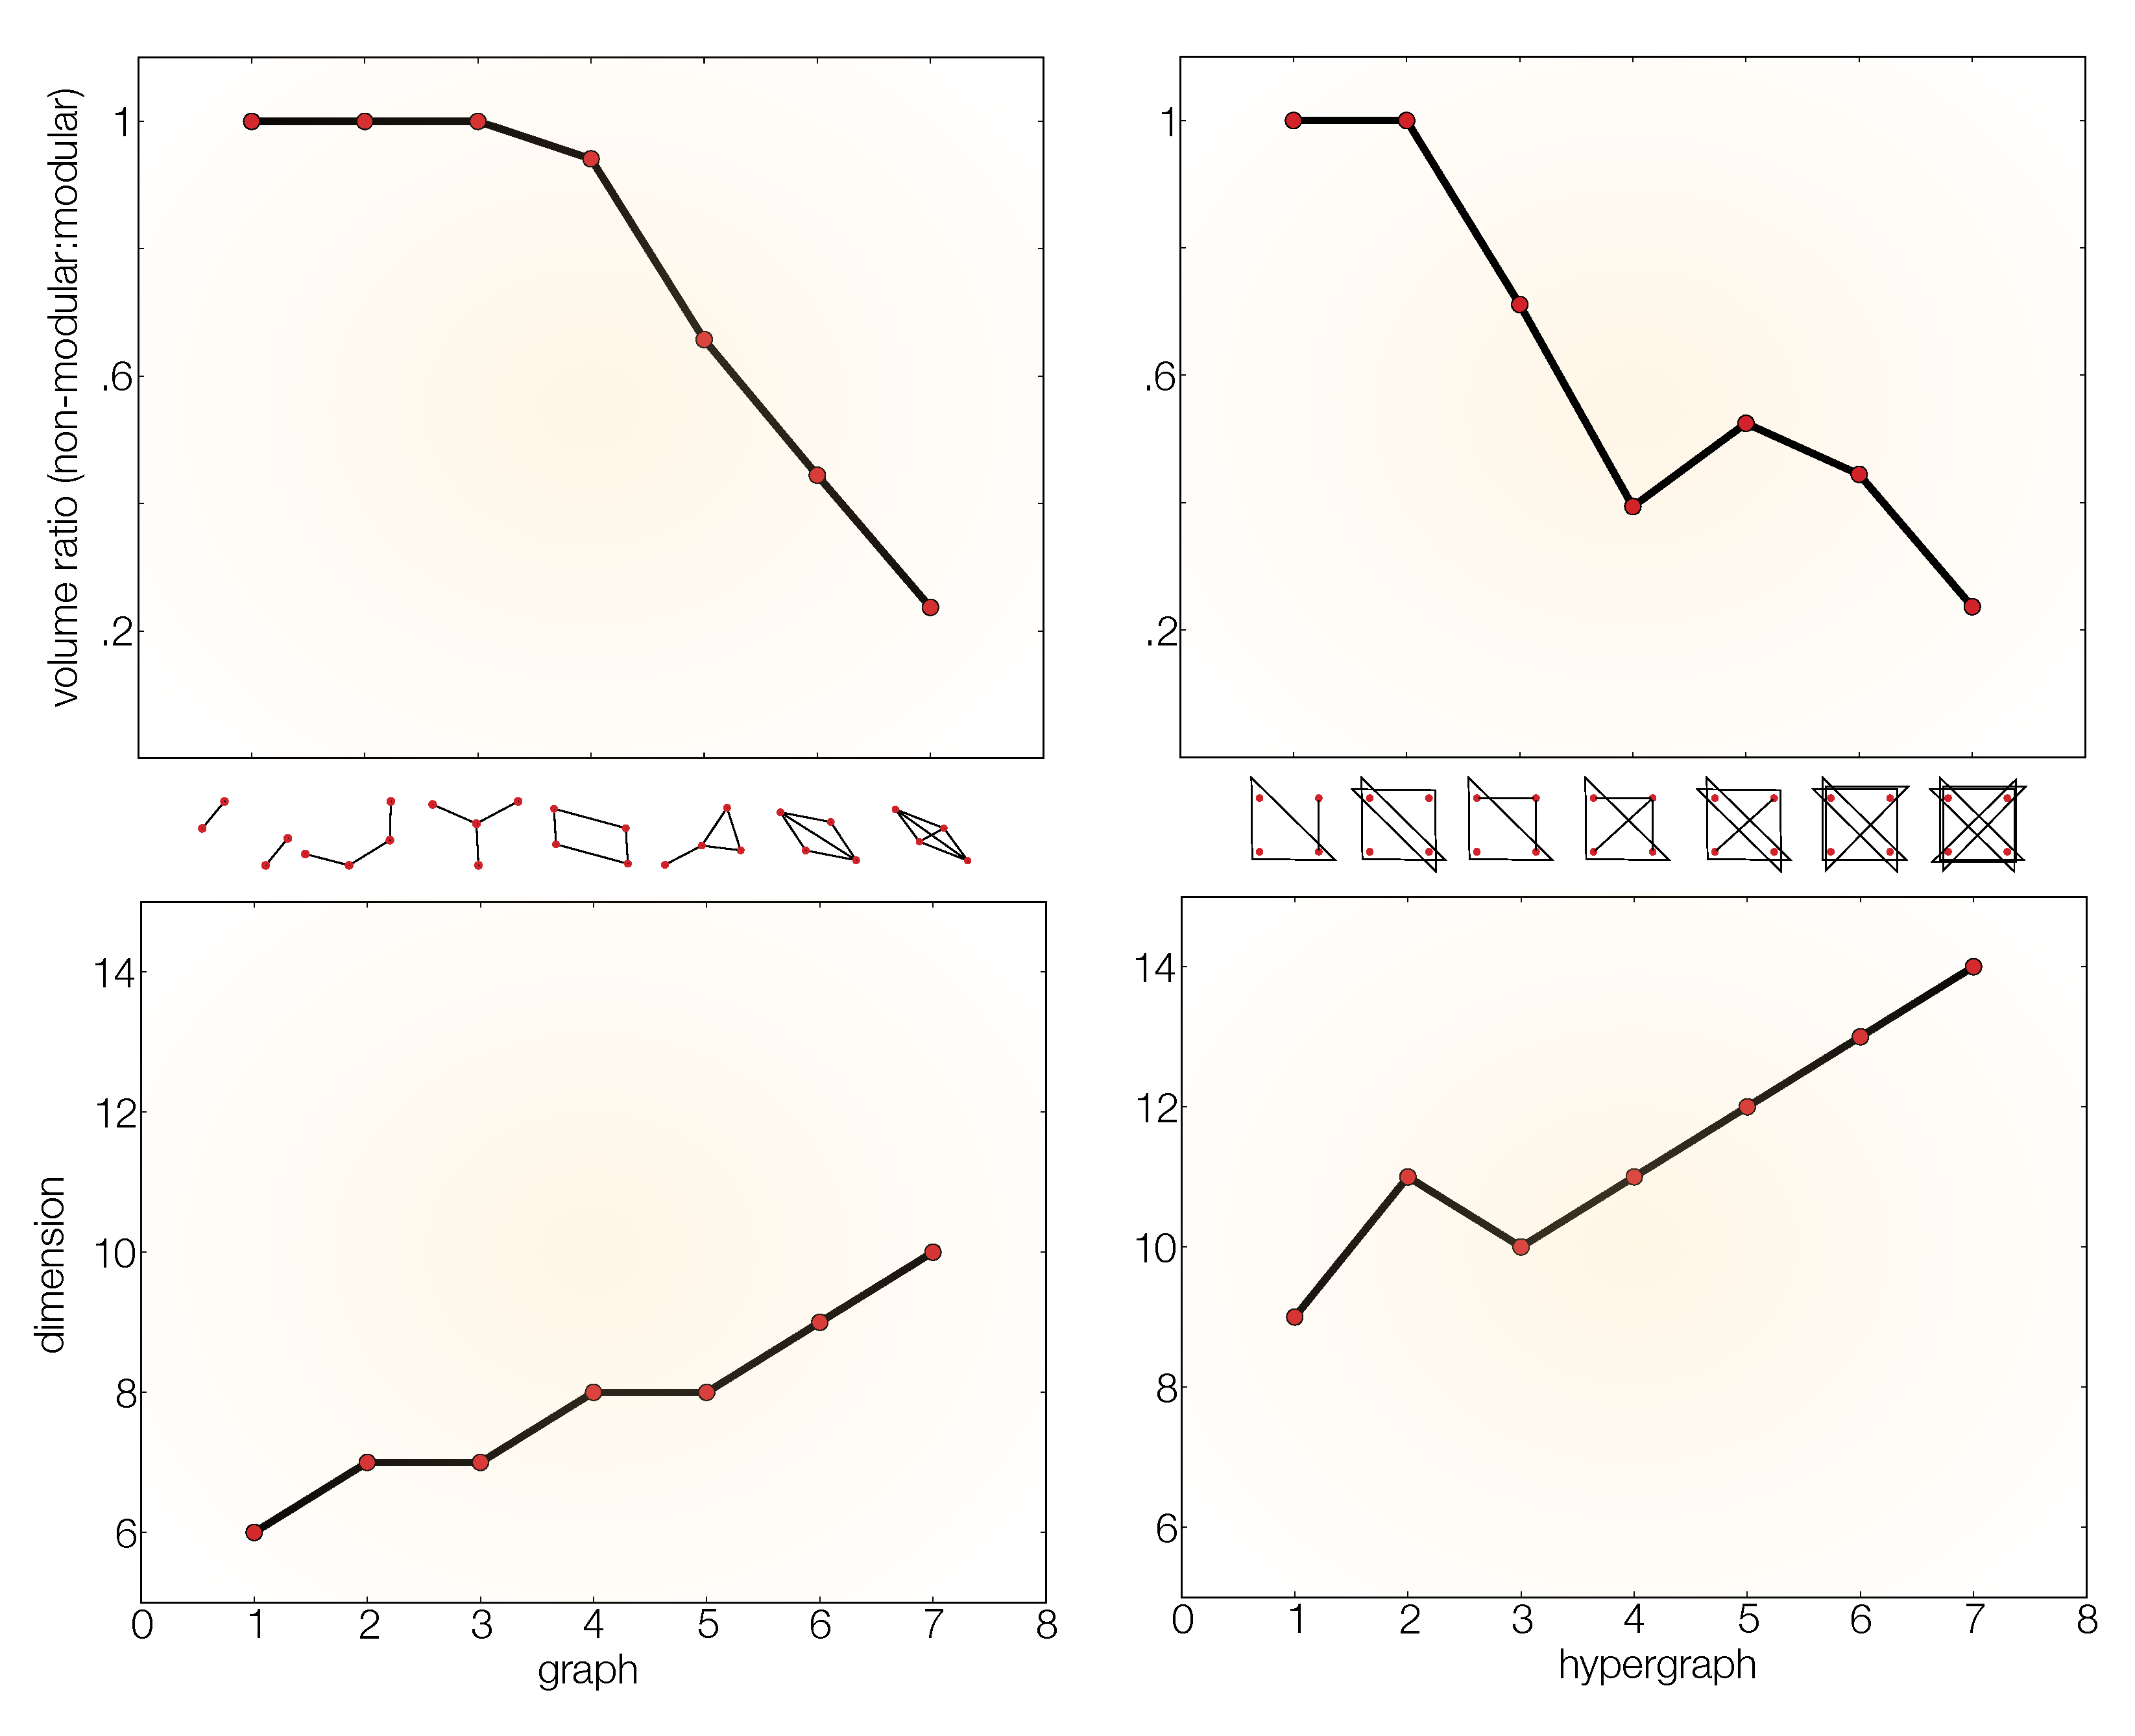
\includegraphics[width=0.9\columnwidth]{fig/figure_graphs_dims_nolines.pdf}
\caption{{\bf Non-modular to modular probability space volume ratio.} (A) and (B) show the ratio $\frac{\text{Vol}(\mathbb{M}(\mathcal{G}))}{\text{Vol}(\mathbb{L}(\mathcal{G}))}$ associated to 2-regular and non-2-regular network architectures respectively. The (hyper)graph associated to each value of the volume ratio is displayed along the x-axis of each panel. (C) and (D) show the natural dimension of the space of probability distributions associated to $\mathbb{M}(\mathcal{G})$ and $\mathbb{L}(\mathcal{G})$ for each hypergraph.}
\label{fig:ncycvolrat}
\end{figure}

\begin{figure}[!ht]
\centering
\noindent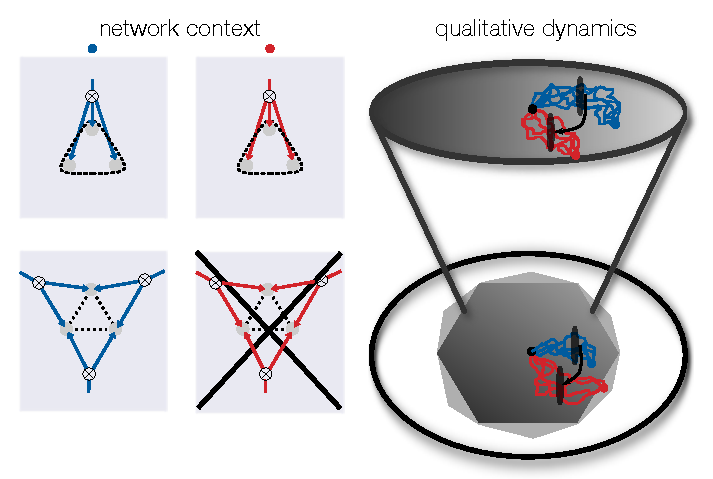
\includegraphics[width=0.9\columnwidth]{fig/stochdynscheme.pdf}
\caption{{\bf Constraints imposed on stochastic biological networks and evolutionary dynamics by network architecture.} Schematic representation of a potential network context (left) for each of the hypothetical stationary probability distributions associated to the fitness peak established by the blue and red points within the spaces of probability distributions represented on the right.
%Algebraically, the top one corresponds to $\dist (\expr (L))$ and the bottom to $\dist (\expr (\mathcal{G}))$.
Either of the two network architectures represented on the left are capable of achieving the stationary distribution over \gnpm{} specified by the blue stationary distribution associated to a hypothetical fitness peak. On the other hand, only the network architecture from the top (and not the bottom) is capable of achieving the red stationary distribution representing an alternative potential fitness peak.}
\label{fig:stochdynscheme}
\end{figure}
